% Chapter 4 - Design

\glsresetall % reset the glossary to expand acronyms again
\chapter[Design]{Design}\label{ch:Design}
\index{Design}

\section{Introduction}
\label{sec:DesignIntroduction}

The purpose of this chapter will be to present, in detail, the design of a smart sunbird feeder. The design explained in this chapter will build on the information presented in the previous chapters. The design approach used for this system follows the methodology and design decisions established in Chapter~\ref{ch:Methodology}. As this system comprises of several hardware and software subsystems, this chapter will describe each subsystem in its own subsection. 

\section{Hardware Design}
\label{sec:HardwareDesign}

This section details the design of the physical/material subsystems and components of which the system is comprised. Overall, the subsystems comprising of the system's hardware are connected to each other through electrical and communication interfaces. The interaction between all of the hardware subsystems is represented in Figure~\ref{fig:hardware_block_diagram}, which shows the power and signal connections between each of the components. The hardware design of the system is presented in the following subsections, which include the feeder and mechanical design, embedded computing and camera, visit-detection hardware, storage and hardware interfaces, power and solar system, and enclosure and outdoor installation.

\begin{figure}[htbp]
\centering
\resizebox{\textwidth}{!}{%
\begin{tikzpicture}[
    >=Latex,
    font=\sffamily,
    block/.style={
        rectangle,
        draw,
        thick,
        rounded corners=2pt,
        minimum height=2.2cm
    },
    camerablock/.style={block, fill=blue!15, minimum width=4.2cm},
    sensorblock/.style={block, fill=green!20, minimum width=6.4cm},
    computerblock/.style={block, fill=orange!20, minimum width=6.4cm, minimum height=3.0cm},
    powerblock/.style={block, fill=yellow!25, minimum width=4.6cm},
    title/.style={font=\sffamily\bfseries\small, align=center},
    pin/.style={font=\sffamily\scriptsize, inner sep=1.5pt, align=center},
    signal/.style={font=\sffamily\scriptsize, fill=white, inner sep=1.5pt},
    wire/.style={->, thick},
    group/.style={draw, thick, inner sep=0.45cm},
    grouplabel/.style={font=\sffamily\bfseries\small, anchor=north west, inner sep=4pt}
]

% ---------------------------------------------------------------- Blocks
\node[sensorblock]   (tof)   at (6.8,  3.2) {};
\node[camerablock]   (cam)   at (0.0,  0.2) {};
\node[computerblock] (pi)    at (6.8, -3.2) {};
\node[powerblock]    (solar) at (14.6, 3.2) {};
\node[powerblock, minimum height=3.0cm] (psu) at (14.6,-3.2) {};

% ---------------------------------------------------------------- Titles
\node[title, below=3pt of tof.north]   {VL53L1X TIME-OF-FLIGHT\\DISTANCE SENSOR};
\node[title, below=3pt of cam.north]   {PI CAMERA\\MODULE V3};
\node[title, above=3pt of pi.south]    {RASPBERRY PI 4B};
\node[title, below=3pt of solar.north] {MC 12\,V SOLAR\\PANEL};
\node[title, above=3pt of psu.south]   {WAVESHARE SOLAR\\POWER MANAGER B};

% ---------------------------------------------------------------- Pins
% ToF sensor (bottom edge)
\node[pin, anchor=south] (tofVIN) at ($(tof.south west)!0.1!(tof.south east)$) {VIN};
\node[pin, anchor=south] (tofGND) at ($(tof.south west)!0.3!(tof.south east)$) {GND};
\node[pin, anchor=south] (tofSDA) at ($(tof.south west)!0.5!(tof.south east)$) {SDA};
\node[pin, anchor=south] (tofSCL) at ($(tof.south west)!0.7!(tof.south east)$) {SCL};
\node[pin, anchor=south] (tofINT) at ($(tof.south west)!0.9!(tof.south east)$) {GPIO1};

% Camera module (bottom edge)
\node[pin, anchor=south] (cam3v3) at ($(cam.south west)!0.2!(cam.south east)$) {CAM\_3v3};
\node[pin, anchor=south] (camGND) at ($(cam.south west)!0.5!(cam.south east)$) {GND};
\node[pin, anchor=south] (camIO)  at ($(cam.south west)!0.8!(cam.south east)$) {CAM\_GPIO};

% Raspberry Pi (top edge)
\node[pin, anchor=north] (pi3V3)  at ($(pi.north west)!0.1!(pi.north east)$) {3V3\\(PIN 1)};
\node[pin, anchor=north] (piGND)  at ($(pi.north west)!0.3!(pi.north east)$) {GND\\(PIN 6)};
\node[pin, anchor=north] (piSDA)  at ($(pi.north west)!0.5!(pi.north east)$) {GPIO 2\\(PIN 3)};
\node[pin, anchor=north] (piSCL)  at ($(pi.north west)!0.7!(pi.north east)$) {GPIO 3\\(PIN 5)};
\node[pin, anchor=north] (piGPIO) at ($(pi.north west)!0.9!(pi.north east)$) {GPIO 17\\(PIN 11)};
% Raspberry Pi (left edge)
\node[pin, anchor=west]  (piCSI5)   at ($(pi.north west)!0.40!(pi.south west)$) {CSI\_5};
\node[pin, anchor=west]  (piCSIGND) at ($(pi.north west)!0.58!(pi.south west)$) {GND};
\node[pin, anchor=west]  (piCSI3v3) at ($(pi.north west)!0.76!(pi.south west)$) {CSI\_3v3};
% Raspberry Pi (right edge)
\node[pin, anchor=east]  (piUSB)    at ($(pi.north east)!0.45!(pi.south east)$) {USBC\_IN};

% Solar panel (bottom edge)
\node[pin, anchor=south] (solOUT) at ($(solar.south west)!0.25!(solar.south east)$) {V\_OUT};
\node[pin, anchor=south] (solGND) at ($(solar.south west)!0.75!(solar.south east)$) {GND};

% Power manager (top and left edges)
\node[pin, anchor=north] (psuIN)  at ($(psu.north west)!0.25!(psu.north east)$) {V\_IN};
\node[pin, anchor=north] (psuGND) at ($(psu.north west)!0.75!(psu.north east)$) {GND};
\node[pin, anchor=west]  (psuOUT) at ($(psu.north west)!0.45!(psu.south west)$) {USB\_OUT};

% ---------------------------------------------------------------- Connections
% Raspberry Pi <-> ToF sensor (I2C bus plus interrupt line)
\draw[wire] (pi3V3.north |- pi.north) -- node[signal] {3.3\,V} (tofVIN.south |- tof.south);
\draw[wire] (piGND.north |- pi.north) -- (tofGND.south |- tof.south);
\draw[wire, <->] (piSDA.north |- pi.north) -- node[signal, pos=0.35] {I\textsuperscript{2}C data} (tofSDA.south |- tof.south);
\draw[wire] (piSCL.north |- pi.north) -- node[signal, pos=0.65] {I\textsuperscript{2}C clock} (tofSCL.south |- tof.south);
\draw[wire] (tofINT.south |- tof.south) -- node[signal] {interrupt} (piGPIO.north |- pi.north);

% Raspberry Pi <-> camera module (CSI ribbon)
\draw[wire] (camIO.south |- cam.south) |- (piCSI5.west -| pi.west);
\draw[wire] (piCSIGND.west -| pi.west) -| (camGND.south |- cam.south);
\draw[wire] (piCSI3v3.west -| pi.west) -- ++(-1.2,0) node[signal, midway, above] {3.3\,V}
            -| (cam3v3.south |- cam.south);

% Solar panel <-> power manager
\draw[wire] (solOUT.south |- solar.south) -- node[signal] {12\,V} (psuIN.north |- psu.north);
\draw[wire] (psuGND.north |- psu.north) -- (solGND.south |- solar.south);

% Power manager -> Raspberry Pi
\draw[wire] (psuOUT.west -| psu.west) -- node[signal] {5\,V} (piUSB.east -| pi.east);

% ---------------------------------------------------------------- Groupings
\begin{scope}[on background layer]
    % Extra headroom above each group leaves space for its label
    \node[group, fit={(cam) (tof) (pi) ($(tof.north)+(0,0.4)$)}] (embedded) {};
    \node[group, fit={(solar) (psu) ($(solar.north)+(0,0.4)$)}] (power) {};
    \node[group, fit={(embedded) (power) ($(embedded.north)+(0,0.4)$)}, inner sep=0.3cm] (hardware) {};
\end{scope}
\node[grouplabel] at (embedded.north west) {EMBEDDED SYSTEM};
\node[grouplabel] at (power.north west)    {POWER};
\node[grouplabel] at (hardware.north west) {HARDWARE};

\end{tikzpicture}%
}
\caption{Hardware interfacing diagram of the smart sunbird feeder, showing the hardware subsystems and the power and signal connections between them.}
\label{fig:hardware_block_diagram}
\end{figure}

\subsection{Feeder and Mechanical Design}
\label{subsec:FeederMechanicalDesign}

% \begin{itemize}
%     \item Describe the nectar-feeder arrangement.
%     \item Explain bird positioning relative to the feeder and camera.
%     \item Describe the feeder mounting method and measures used to reduce sway.
%     \item Discuss accessibility for cleaning and refilling.
%     \item Consider mechanical robustness and outdoor suitability.
% \end{itemize}

As previously mentioned in Chapter~\ref{ch:LitReview} and Chapter~\ref{ch:Methodology}, sunbirds are nectar-feeding birds. The proper storage and maintainence of a nectar feeder are key considerations when selecting the feeding mechanism. The nectar is reuired to be replaced every 48 hours at most, with its container being cleaned at similar intervals to remain hygenic and safe for bird use. These requirements translate to a need for an easily-accessible feeder that is robust to environmental factors and is capable of storing liquid reliably and without risk of contamination.

Due to these intricate requirements of the feeder for this project, it was decided that this project will utilize a very simple, commercially available nectar feeder. The feeder selected for this project was chosen for its simplicity, availability, cost-effectiveness and proven satisfaction of all necessary concerns of reliability and safety. The feeder used for this project, a 750\,ml sunbird nectar feeder from Stodels \cite{StodelsSunbirdFeeder}, is shown in Figure~\ref{fig:stodels_nectar_feeder}.

\begin{figure}[htbp]
\centering
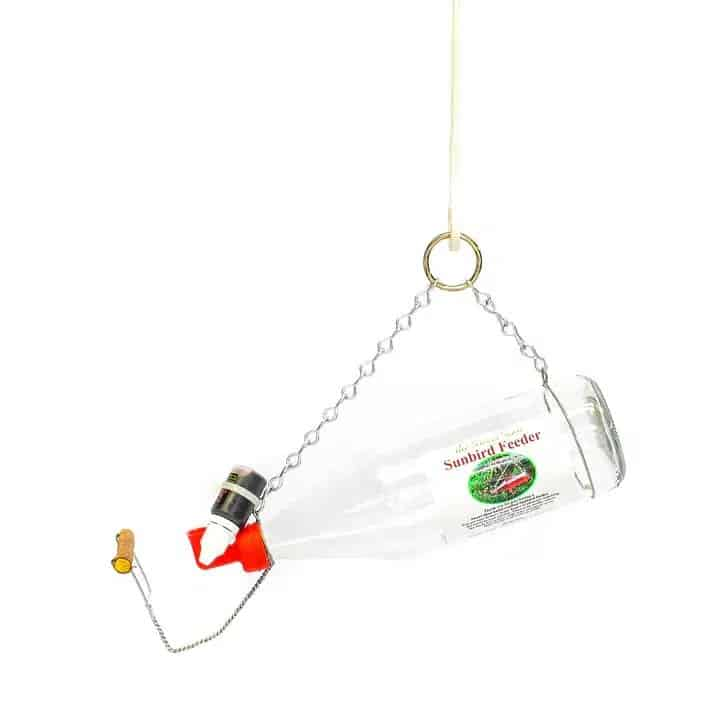
\includegraphics[width=0.4\textwidth]{3_Chapters/4_Chapter_Design/Figures/stodels_nectar_feeder.jpg}
\caption{The commercially available Stodels 750\,ml sunbird nectar feeder used in this project \cite{StodelsSunbirdFeeder}.}
\label{fig:stodels_nectar_feeder}
\end{figure}

This project required multiple additional components to be physically connected to the feeder. The stock feeder selected for this project offered little purchase for such components to be attached between its smooth glass body and minimal chain support mechanism. For this reason, it was decided to remove the chains entirely from the glass bottle and integrate the bottle into a larger housing that better accommodated for the introduction of the extra components required. The design of this housing is documented further in Section~\ref{subsec:EnclosureOutdoorDesign}.

\subsection{Embedded Computing and Camera}
\label{subsec:EmbeddedCameraDesign}

\begin{itemize}
    \item Present the selected embedded computing platform.
    \item Present the selected camera module.
    \item Describe the relevant interfaces between the camera and embedded computer.
    \item Include important technical specifications relevant to system operation.
    \item Explain how the selected hardware satisfies the processing and imaging requirements of the project.
\end{itemize}


\subsection{Visit-Detection Hardware}
\label{subsec:VisitDetectionHardware}

\begin{itemize}
    \item Describe any sensor hardware used to detect or trigger bird visits.
    \item Explain sensor positioning and connection to the embedded computing platform.
    \item Discuss relevant detection range, response and interface considerations.
    \item If visit detection is implemented entirely in software, move the relevant discussion to Section~\ref{sec:SoftwareDesign}.
\end{itemize}


\subsection{Storage and Hardware Interfaces}
\label{subsec:StorageHardwareInterfaces}

\begin{itemize}
    \item Describe the local storage hardware used by the system.
    \item Present the main electrical and communication interfaces between components.
    \item Include a simplified hardware connection diagram where appropriate.
    \item Discuss any supporting electronics required for system operation.
\end{itemize}


\subsection{Power and Solar System}
\label{subsec:PowerSolarDesign}

\begin{itemize}
    \item Present the overall power architecture.
    \item Describe the battery, solar panel, charge controller and voltage-regulation components.
    \item Explain power distribution to the embedded computer and peripherals.
    \item Include provision for manual charging where applicable.
    \item Present relevant sizing calculations or design equations where necessary.
\end{itemize}


\subsection{Enclosure and Outdoor Installation}
\label{subsec:EnclosureOutdoorDesign}

\begin{itemize}
    \item Describe the enclosure used for the electronics and power components.
    \item Explain protection against rain, moisture, dust and direct environmental exposure.
    \item Discuss ventilation and thermal considerations.
    \item Describe the mounting arrangement for the electronics, battery and solar panel.
\end{itemize}


\section{Software Design}
\label{sec:SoftwareDesign}

\subsection{Software Architecture}
\label{subsec:SoftwareArchitecture}

\begin{itemize}
    \item Present the overall software architecture.
    \item Include a software block diagram or flow diagram.
    \item Identify the main software modules and their interactions.
\end{itemize}


\subsection{Visit Detection and Video Capture}
\label{subsec:VisitDetectionVideoCapture}

\begin{itemize}
    \item Describe the software logic used to detect or respond to a bird visit.
    \item Explain how video recording is initiated and terminated.
    \item Describe how recorded visits are separated and stored.
    \item Explain the handling of repeated or false triggers where relevant.
\end{itemize}


\subsection{Video Processing and Species Identification}
\label{subsec:VideoProcessingSpeciesID}

\begin{itemize}
    \item Describe how recorded video is processed prior to inference.
    \item Explain the frame-selection method.
    \item Describe any image preprocessing.
    \item Present the selected species-classification model.
    \item Define the locally relevant classification classes.
    \item Explain inference and confidence handling.
    \item Describe how multiple frame predictions are combined into a visit-level result where applicable.
\end{itemize}


\subsection{Data Logging and Storage}
\label{subsec:DataLoggingStorage}

\begin{itemize}
    \item Describe how visit information is logged.
    \item Present the database structure at an appropriate level of detail.
    \item Describe the storage of:
    \begin{itemize}
        \item Date and time.
        \item Video file location.
        \item Predicted species.
        \item Classification confidence.
        \item Visit duration.
        \item Processing status.
        \item Relevant system logs.
    \end{itemize}
\end{itemize}


\subsection{Web Interface}
\label{subsec:WebInterfaceDesign}

\begin{itemize}
    \item Describe the local web-interface architecture.
    \item Explain interaction between the web server, database and stored video files.
    \item Present the main interface functions, including:
    \begin{itemize}
        \item Dashboard.
        \item Recent visit history.
        \item Species-identification results.
        \item Video playback.
        \item Basic system status.
        \item Relevant settings where implemented.
    \end{itemize}
\end{itemize}


\subsection{System Control and Reliability}
\label{subsec:SystemControlReliability}

\begin{itemize}
    \item Describe software mechanisms used to support reliable unattended operation.
    \item Discuss relevant features such as:
    \begin{itemize}
        \item Automatic startup.
        \item Error handling.
        \item Process recovery.
        \item Storage management.
        \item System logging.
        \item Power-aware operation.
    \end{itemize}
    \item Omit this subsection if these functions are more appropriately discussed within the preceding software subsections.
\end{itemize}


\section{System Integration}
\label{sec:SystemIntegration}

\begin{itemize}
    \item Explain how the hardware, software, mechanical and power subsystems are combined.
    \item Present the final integrated system architecture.
    \item Include photographs or annotated diagrams of the completed system where appropriate.
    \item Discuss any important integration constraints or modifications.
    \item Avoid repeating detailed subsystem descriptions already presented earlier in the chapter.
\end{itemize}


\section{Bill of Materials}
\label{sec:BillOfMaterials}

\begin{itemize}
    \item Present the main components used in the completed system.
    \item Include:
    \begin{itemize}
        \item Component.
        \item Quantity.
        \item Function.
        \item Supplier or source.
        \item Unit cost.
        \item Total cost.
    \end{itemize}
    \item Group components into mechanical, electronic and power categories where useful.
\end{itemize}

% Example table structure:
%
% \begin{table}[ht]
% \centering
% \caption{Bill of materials for the smart sunbird feeder}
% \label{tab:BillOfMaterials}
% \begin{tabular}{lclrr}
% \hline
% \textbf{Component} & \textbf{Qty.} & \textbf{Supplier} &
% \textbf{Unit Cost} & \textbf{Total Cost} \\
% \hline
% Raspberry Pi & 1 & -- & R-- & R-- \\
% Camera Module & 1 & -- & R-- & R-- \\
% Battery & 1 & -- & R-- & R-- \\
% Solar Panel & 1 & -- & R-- & R-- \\
% \hline
% \end{tabular}
% \end{table}


\section{Conclusion}
\label{sec:DesignConclusion}

\begin{itemize}
    \item Summarise the completed system design.
    \item Reinforce how the hardware and software subsystems combine into a functional smart sunbird feeder.
    \item Relate the final design back to the main system requirements.
    \item Transition to the subsequent chapter covering system testing, results and evaluation.
\end{itemize}